\documentclass[12pt]{article}
\usepackage[english]{babel}
\usepackage{natbib}
\usepackage{url}
\usepackage[utf8x]{inputenc}
\usepackage{amsmath}
\usepackage{graphicx}
\graphicspath{{images/}}
\usepackage{parskip}
\usepackage{fancyhdr}
\usepackage{vmargin}
\usepackage{subfig}
\usepackage{float}
\setmarginsrb{3 cm}{2.5 cm}{3 cm}{2.5 cm}{1 cm}{1.5 cm}{1 cm}{1.5 cm}

\title{2.1 - Differential Amplifier (Prelab)}                             % Title
\author{John Wu \\ Ian Smith \\ Bilal Yousuf}                               % Author
\date{\today}                                                           % Date

\makeatletter
\let\thetitle\@title
\let\theauthor\@author
\let\thedate\@date
\makeatother

\pagestyle{fancy}
\fancyhf{}
\rhead{\theauthor}
\lhead{\thetitle}
\cfoot{\thepage}

\begin{document}

%%%%%%%%%%%%%%%%%%%%%%%%%%%%%%%%%%%%%%%%%%%%%%%%%%%%%%%%%%%%%%%%%%%%%%%%%%%%%%%%%%%%%%%%%

\begin{titlepage}
    \centering
    \vspace*{0.5 cm}
    
\includegraphics[scale = 0.07]{mcgill-logo.png}\\[1.0 cm]   % University Logo
    \textsc{\LARGE McGill University}\\[1.0 cm]   % University Name
    \textsc{\Large ECSE 335}\\[0.5 cm]               % Course Code
    \textsc{\large Microelectronic Labs}\\[0.5 cm]               % Course Name
    \rule{\linewidth}{0.2 mm} \\[0.4 cm]
    { \huge \bfseries \thetitle}\\
    \rule{\linewidth}{0.2 mm} \\[1.5 cm]
    \begin{minipage}{0.4\textwidth}
        \begin{flushleft} \large
            \emph{Authors (Group X):}\\
            \theauthor
            \end{flushleft}
            \end{minipage}~
            \begin{minipage}{0.4\textwidth}
            \begin{flushright} \large
            \emph{Student Number:} \\
            260612056 \\ 260612056 \\ 260680182                                  % Your Student Number
        \end{flushright}
    \end{minipage}\\[2 cm]
 
    {\large \thedate}\\[2 cm]
 
    \vfill
    
\end{titlepage}

%%%%%%%%%%%%%%%%%%%%%%%%%%%%%%%%%%%%%%%%%%%%%%%%%%%%%%%%%%%%%%%%%%%%%%%%%%%%%%%%%%%%%%%%%

\section*{2.1 Preparation}

\begin{figure}[H]
\centering
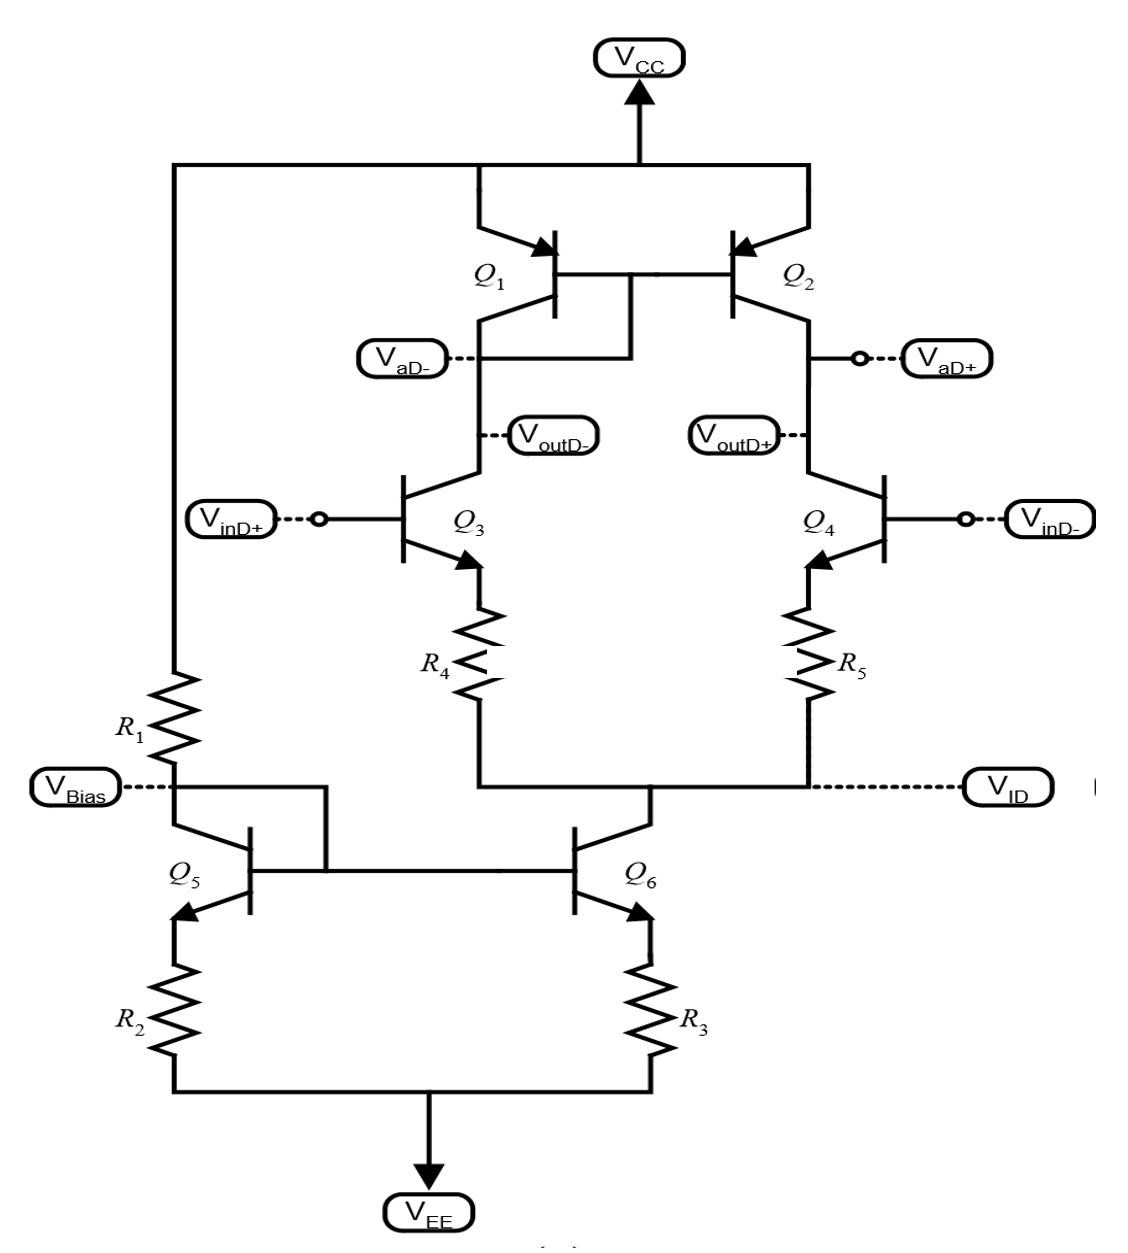
\includegraphics[width=0.6\textwidth]{op_amp.PNG}
\caption{\label{fig:op-amp} Differential amplifier with active load}
\end{figure}

\subsection*{2.1.2 Considering this circuit will be used as an output stage in an operational amplifier, what are the main characteristics that it must have?}

Since the circuit will be used as an output stage in an operational amplifier, it must have the following characteristics in its most ideal form.


\begin{itemize}
    \item Infinite open-loop gain.
    \item Infinite bandwidth due to ideal gain.
    \item Infinite or zero common mode rejection ratio (CMRR).
    \item Infinite input impedance.
    \item Zero output impedance.
\end{itemize}

In general, these ideal characteristics will not be the actual case, but it will aim to be as close to these idealistic values as possible in order to deliver large currents to a small load - the goal of an op-amp.

\subsection*{2.1.3 What is the purpose of $R_2$ and $R_3$?}

The resistors, $R_2$ and $R_3$, are source degeneration resistances used for creating a higher output impedance and a lower equivalent transconductance. These resistors are used to give a high resistance to the current mirror formed by $Q_5$ and $Q_6$. The high output resistance will reduce the common mode gain and improve the CMRR. The resistors prevent thermal runaway in transistors Q5 and Q6 thereby providing thermal stability.

\subsection*{2.1.4 Using $V_{EE} = -5V$ and $V_{CC} = 5V^1$, design the current source of the differential pair so that it sinks a current of $0.25mA$. Determine the required value of $R$.}

When $R_2 = R_3 = 2k\Omega$ and $Q_5$ and $Q_6$ make perfect current mirrors: \\

$I = \frac{V_{EE} - V_{BE} - V_{CE}}{R_2 + R_1}$ \\

$\frac{9.3V}{2k\Omega + R_1} = 0.25mA$ \\

$R_1 = 35.2k\Omega$


\subsection*{2.1.5 Considering the current source only, plot the source’s output current versus the output voltage and comment on the results.}

\begin{figure}[H]
\centering
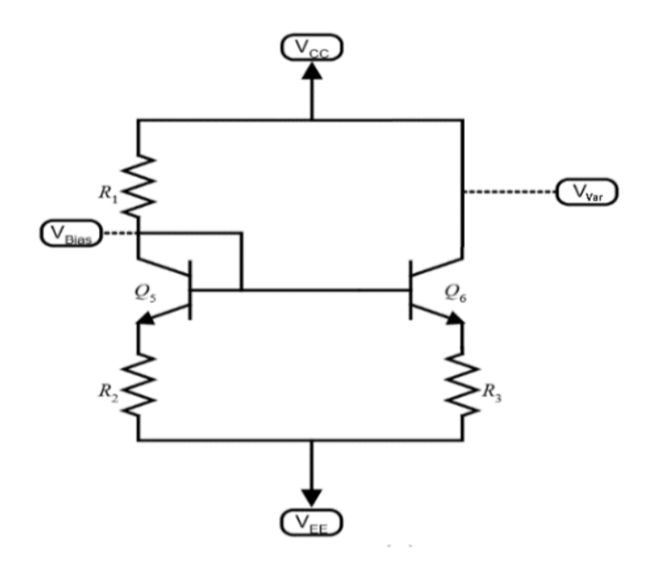
\includegraphics[width=0.5\textwidth]{current_source.PNG}
\caption{\label{fig:current-source} Circuit used for analyzing current source.}
\end{figure}

\subsection*{2.1.6 Design the circuit of Figure 2.1 in order to obtain a gain of $250V/V ±10\%$. Determine the values of $R_4$ and $R_5$. Discuss. At the output, take into account the loading caused by a $10X$ oscilloscope probe.}

$r_e = \frac{V_T}{I_C} = \frac{25mV}{0.125mA} = 200\Omega$ \\
\\$r_{o2} = \frac{V_A}{I_C} = \frac{115.7V}{0.125mA} = 925.6k\Omega$\\
\\$r_{o4} = \frac{V_A}{I_C} = \frac{74.03V}{0.125mA} = 592.24k\Omega$\\
\\$g_m = \frac{I_C}{V_T} = \frac{0.125mA}{25mV} = 5mA/V$\\
\\$A_d = \frac{r_{o4}(1+g_mR_4)||r_{o2}||R_{OSC}}{r_e + R_4}$\\
\\$R_4$ is approximately $2.9k\Omega$. We'll make $R_5 = R_4 = 2.9k\Omega$\\

\subsection*{2.1.7 Plot the voltage transfer characteristics and accompany it with the corresponding time domain waveform plot. Discuss the curve and maximal output swing.}

INSERT ANSWER HERE

\subsection*{2.1.8 Determine, if any, the input DC offset required to maximize the output swing. Document the maximum output swing. Discuss.}

INSERT ANSWER HERE

\subsection*{2.1.9 Plot the differential mode frequency response and determine the $3-dB$ points. Also, take into account the parasitic resistor and capacitor values of the $10X$ oscilloscope probe at the output. Discuss.  }

INSERT ANSWER HERE

\subsection*{2.1.10 Plot the common mode frequency response. Also, take into account the parasitic resistor and capacitor values of the $10X$ oscilloscope probe at the output. Discuss. }

\subsection*{2.1.11 Find the input and output resistances the circuit. Discuss. }

INSERT ANSWER HERE

\subsection*{2.1.12 In summary, what are the advantages and limitations of this circuit setup?}

\begin{figure}[H]
  \centering
    \subfloat[]{{\includegraphics[width=0.4\textwidth]{image1.jpg} }}%
    \qquad
    \subfloat[]
    {{\includegraphics[width=0.4\textwidth]{image2.jpg} }}%
    \qquad
    \caption{sample image with caption}%      
    \label{fig:testing}%
\end{figure}


\end{document}